\section{Modelling}
A model of each individual circuit component is fabricated. This is used to provide a model of the circuit as a whole, using nodal analysis methods .i.e. Krichoff's Laws

\subsection{Component Values}
The values of the circuit components are presented in the table below. Where there is an applicable tolerance level, the maximum and minimum values are shown. 
\begin{table}[H]
    \centering
    \begin{tabular}{|c|c|c||c|c|}\hline
        & Value & \% Tolerance & \textbf{Maximum} & \textbf{Minimum} \\\hline
       $C$ & $0.0022 F$ & $20\%$ & $0.00264F$ & $0.00176F$ \\
       $R_s$ & $300\Omega$ & $10\%$ & $330\Omega$ & $270\Omega$ \\
       $R_{L_1}$ & $65.7\Omega$ & $0\%$ & $65.7\Omega$  & $65.7\Omega$ \\
       $R_{L_2}$ & $287\Omega$ & $0\%$ & $287\Omega$ & $287\Omega$ \\
       $R_b$ & $3.2 \Omega$ & $0\%$ & $3.2 \Omega$ & $3.2 \Omega$ \\
       $R_z$ & $4.85 \Omega$ & $0\%$ & $4.85 \Omega$ & $4.85 \Omega$ \\
       $V_z$ & $6.2 V$ & $0\%$ & $6.2 V$ & $6.2 V$ \\
       $L$ & $0.01058 H$ & $0\%$ & $0.01058 H$ & $0.01058 H$ \\\hline
    \end{tabular}
    \caption{Circuit component values and their variances}
    \label{tab:component_values}
\end{table}
where,
\begin{itemize}
	\item $C$ is the capacitance value of the capacitor connected to the rectifier
	\item $R_s$ is the resistance value of the resistor parallel to the capacitor
	\item $R_{L_1}, R_{L_2}$ are one of the resistance values of the multi-mode load
	\item $R_b$ is the bulk resistance of the ideal diode
	\item $L$ is the inductance of the load
	\item $R_z$ is the breakdown resistance of the zener diode
	\item $V_z$ is the breakdown voltage of the zener diode
\end{itemize}

\pagebreak
\subsection{Component Modelling}
Each individual component in the circuit must be represented analytically. Circuit components are assumed to be ideal, .i.e. there is an absence of source resistance and or impedance. The model does not account for inexactitudes in component values that may be realised in a practical implementation. 

\subsubsection{Voltage Source} The voltage source is modelled as an ideal AC voltage source. There is no source impedance, thus, we assume that the source generates the exact amount of voltage across its terminals. 
\begin{equation}
    \begin{split}
        V_{\text{in}} &= V_{\text{rms}}\sqrt{2}\text{sin}(\omega t + \phi)
            \\ &= 230\sqrt{2}\text{sin}(100\pi t)V
    \end{split}
\end{equation}
where $V_{\text{rms}}$ is the rms voltage, $\omega = 2\pi f$ is the angular frequency

\subsubsection{Capacitor} The capacitor is modelled as an ideal capacitor that does not dissipate energy. The current across the capacitor is given by:
\begin{equation}
    i = C \frac{dV}{dt}
    \label{eq:ideal_capacitor}
\end{equation}
where $C$ is the capacitance in Farads (F), $\frac{dV}{dt}$ is the rate of change of voltage $\left(\frac{V}{s}\right)$

\subsubsection{Inductor} The inductor is modelled as an ideal inductor whose voltage is given by:
\begin{equation}
    V = L\frac{di}{dt}
    \label{eq:ideal_inductor}
\end{equation}
where $L$ is the inductance in Henry's, $\frac{di}{dt}$ is the rate of current change
\subsubsection{Resistor} The resistor is modelled as an ideal resistor whose voltage is given by Ohm's law
\begin{equation}
    V=IR
\end{equation}
where $V$ is the voltage (V), $I$ is the current (A) and $R$ is the resistance ($\Omega$)

\subsubsection{Switch} The switch is modelled as an ideal switch without any source resistance. The switch can be represented using a binary state .i.e. on or off. It is assumed that there is no propagation delay in the change of state and the effects are immediate. \\

Analytically this can be described as the unit step function $u(t)$,
\begin{equation}
	u(t) = \begin{cases}
		0 \hspace{0.5cm} t < 0, \\
		1 \hspace{0.5cm} t < 1
	\end{cases}
	\label{eq:unit_step_function}
\end{equation}
This represents an instantaneous transition from "off" (0) to "on" (1) at $t=0$, which is the idealised model of a switch operation. 

\begin{figure}[H]
\centering	
\begin{tikzpicture}
\begin{axis}[
    axis lines = middle,
    xlabel = $t$,
    ylabel = {$u(t)$},
    ytick={0,1},
    xtick={-2,0,2},
    ymax = 1.5,
    ymin = -0.5,
    xmax = 3,
    xmin = -3
]
\addplot[
    domain=-3:0, 
    samples=100, 
    color=red,
] {0};
\addplot[
    domain=0:3, 
    samples=100, 
    color=red,
] {1};
\end{axis}
\end{tikzpicture}
\caption{Unit step function $u(t)$}
\end{figure}

\subsubsection{Transformer} The transformer is assumed to be ideal with a turns ratio of $20:1$. The voltage at either side of the transformer can be determined from its common ideal representation
\begin{equation}
    \frac{V_1}{V_2} = \frac{N_1}{N_2}
    \label{eq:ideal_transformer}
\end{equation}
where $N_1=20$ is the number primary turns, $N_2=1$ is the number of secondary turns, $V_1$ is the primary voltage, $V_2$ is the secondary voltage.\\

The voltage at LV-side of the transformer is fed into the full-bridge rectifier. The secondary voltage $V_2$ is given by:
\begin{equation}
    V_2 = \frac{V_1N_2}{N_1} = \frac{V_1}{20}
\end{equation}

\subsubsection{Diode}
The four diodes in the circuit are configured to form a full bridge rectifier. It is assumed all four diodes are identical.

\paragraph{Shockley Ideal Diode}
The diodes can be modelled as a Shockley diode in series with bulk resistance. The Shockley diode model is a simplified model to describe the behaviour of a diode:

\begin{equation}
	I_D = I_s\left( e^{\frac{V_D}{\eta V_T}} - 1 \right) + \frac{V_d}{R_b}	\label{shockeyDiodeWithBulkResistance}
\end{equation}
where,
\begin{itemize}
	\item $I_D$ is the diode current
	\item $I_s$ is the saturation current
	\item $V_D$ is the voltage across the diode
	\item $\eta$ is the ideality factor
	\item $V_T$ is the thermal voltage (determined by $V_T = \frac{KT}{q}$)
	\item $R_b$ is the bulk resistance
\end{itemize}	

The Shockley diode presents a non-linear model of the diode's behaviour which complicates circuit analysis. A piece-wise linear approximation to the DC characteristic of the diode is used for simplicity.

\paragraph{Piece-wise Linear Approximation}
An ideal diode behaves as a switch–conducting current without any losses under forward bias, and completely blocking current under reverse bias. The biasing of a diode is determined by assessing whether the voltage drop across the diode is greater than its threshold voltage ($V_D \geq V_{th}$)

\subparagraph{Ideal Diode}
Assume that the diode is a silicon diode with a threshold voltage of $V_{th} = 0.7 V$. \citep{silicionDiodeThresholdVoltage} The current across diode can be represented analytically as:
\begin{equation}
    i_d = \begin{cases}
        \infty \hspace{1cm} &V_d \geq 0.7V \\
        0 \hspace{1cm}   &V_d < 0.7V
    \end{cases}
    \label{eq:ideal_diode}
\end{equation}
\begin{figure}[H]
    \centering
%    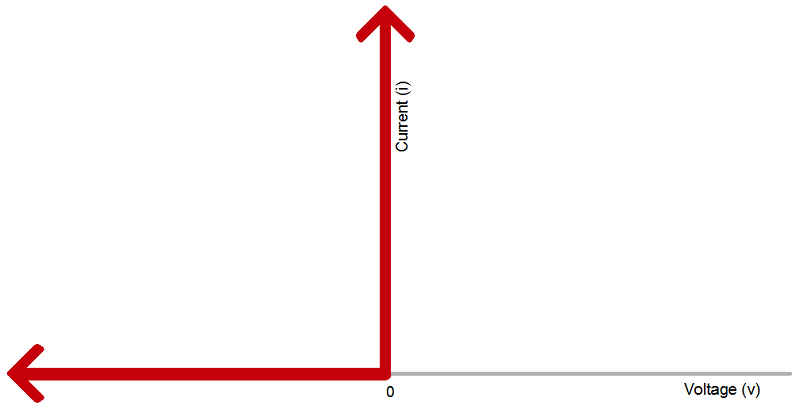
\includegraphics[width=10cm]{graphics/diode_iv.png}
\begin{tikzpicture}
\begin{axis}[
    axis lines = middle,
    xlabel = $V$ (V),
    ylabel = $I$ (A),
    ytick={0,1},
    xtick={-1,0,0.7,1},
    ymax = 1.5,
    ymin = -0.5,
    xmax = 1.5,
    xmin = -1.5
]
\addplot[
    domain=-1.5:0.7, 
    samples=100, 
    color=red,
] {0};
\addplot[
    domain=0.7:1.5, 
    samples=100, 
    color=red,
] {1};
\draw[dashed] (axis cs:0.7,-0.5) -- (axis cs:0.7,1.5) node[pos=0.5, right] {$V_{T}$};
\end{axis}
\end{tikzpicture}
    \caption{The ideal silicon diode i-v characteristic}
    \label{fig:diode_iv_characterstic}
\end{figure}
The diode is represented as a cell ($V_{th}$) in series with a resistor ($R_b$) and an ideal switch. The current flowing into the switch is represented by $i_d$. This is the piece-wise linear approximation of the diode.
\begin{figure}[H]
    \centering
    \begin{circuitikz}[american voltages] \draw
 	(0,5) to[diode,o-o,l=$V_d$,i=$i_d$] (0,0)
	(3,5) to[battery1,o-,l=$V_{th}$] (3,4) 
	(3,4) to[R, l=$R_b$, i_=$i_d$] (3,1)
	(3,1) to[nos,o-o] (3,0);
\end{circuitikz}
    \caption{Piece-wise linear diode approximation of the ideal diode}
    \label{fig:piecewise_diode}
\end{figure}

Analytically $i_d$ can be described using Ohm's law and considering the voltage drop across $R_b$ 
\begin{equation}
    i_d = \begin{cases}
        \bracket{\frac{V_d - V_{th}}{R_b}} \hspace{1cm} &V_d \geq 0.7V \\
        0 \hspace{1cm}   &V_d < 0.7V
    \end{cases}
\end{equation}
This expression matches the expression for the ideal diode presented in \eqref{eq:ideal_diode}. 

\subparagraph{Determination of Maximum Current}\label{determinationOfMaximimumCurrent}
To accurately model the diode using the piece-wise linear circuit in Figure \ref{fig:piecewise_diode}, a reasonable estimate of the maximum current flowing through the diode while it is forward biased must be made.\\

Consider the behaviour of the diode inside the bridge rectifier:

\begin{figure}[H]
	\centering
	
    \begin{circuitikz} [american voltages] \draw
    
    (0,0) to[vsourcesin, l=$V_{in}$] (0,4)
    (0,4) to[battery1, l=$2V_{th}$] (2,4)
    (2,4) to[R,l=$2R_b$,i=$i_d$, v=$V_d$] (7,4)
    (7,4) to[nos,o-o] (8,4)
    (8,4) to[short] (10,4)
    (10,4) to[capacitor, l=$C$,v=$V_c$] (10,0)
    (0,0) to[short] (10,0)
    (5,0) node[ground]{} (5,-1);
    
    \end{circuitikz}
	
	\caption{Piece-wise linear diode model applied in the half-rectifier}
	\label{fig:diode_circuit}
\end{figure}

\begin{itemize}
	\item In a full-bridge rectifier, two diodes are used. One for each half of the cycle (.i.e. half the period of the input sinusoid). \citep{rectifier} Thus, this inequality must be satisfied to ensure forward biasing $$V_d > 2V_{th} = V_d > 1.4V$$
	\item The rectifier is being connected to a capacitor in Figure \ref{fig:powersupply}. When a capacitor is uncharged (.i.e. $V=0$) it behaves as a short circuit. In a DC circuit, the capacitor experiences maximal current at the instant the power supply is connected.
	\item In an AC circuit (.i.e. with a sinusoidal input), the voltage changes over time, so the capacitor does not experience a sudden surge of voltage as it does in the DC circuit.
	\item The maximum charging current occurs during the first peak of the sinusoidal wave, which occurs in the first half cycle: $$0 < t < \frac{T}{2}$$ where T is the period of the sinusoid $T=\frac{1}{f}$
\end{itemize} 

The rate of change of the capacitor voltage ($\frac{dV_c}{dt}$) is the difference across the input and output terminals,
\begin{align}
	\frac{dV_c}{dt} = \frac{V_{in}(t) - 2V_{th} - V_c}{2R_b}
	\label{eq:dvc_dt}
\end{align}
The input voltage $V_{in}(t)$ is stepped down by a factor of 20 due to the rectifier being connected to the LV-side of the ideal transformer (see Figure \ref{fig:powersupply}). Hence it's amplitude $A$ is given by $A = \frac{230\sqrt{2}}{20}$.\\

Substituting \eqref{eq:dvc_dt} into the ideal capacitor model in \eqref{eq:ideal_capacitor}, derive a first-order ODE of $V_c(t)$
\begin{align}
	2R_bC\frac{dV_c}{dt} + V_c(t) = A\text{sin}(\omega t) - 1.4
	\label{eq:diff}
\end{align}
where $A$ is the amplitude of $V_{in}(t)$, $\omega = 100\pi$. To solve the ODE, split it into homogenous and non-homogenous parts. \\

The homogenous part of this equation (.i.e. excluding the sinusoidal term) is:
\begin{equation}
	2R_bC\frac{dV_c}{dt} + V_c(t) = 0
\end{equation}
which has a solution in the form
\begin{equation}
	V_c(t) = Be^{-t\bracket{\frac{1}{2R_bC}}}
\end{equation}
where $B$ is an arbitrary constant to be determined by the initial conditions. 
\\

The non-homogenous part of the equation is defined over the interval $0 \leq t \leq \frac{T}{2}$ and is a sinusoid:
\begin{equation}
	Q\frac{dV_c}{dt} + V_c(t) = A\text{sin}(\omega t) - 1.4
\end{equation}
To find the particular solution, assume a solution in the form:
\begin{equation}
	V_c(t) = M\text{sin}(\omega t) + N\text{cos}(\omega t) 
	\label{vc_t}
\end{equation}
where $M$ and $N$ are arbitrary constants to be determined by initial conditions.\\

The solution to the ODE $V_c(t)$ is the combination of the homogenous and non-homogenous solutions
\begin{equation}
	V_c(t) = Be^{-t\bracket{\frac{1}{2R_bC}}} + M\text{sin}(\omega t) + N\text{cos}(\omega t) - 1.4
\end{equation}
At time $t=0$ the capacitor is uncharged. Thus, the initial condition holds
\begin{equation}
	V_c(0) = 0
	\label{initialCondition}
\end{equation}

Define $p$ as $2R_bC$. The given ordinary differential equation \eqref{eq:diff} can then be written as:
\begin{align}
p\frac{dV_c}{dt} + V_c(t) = A\sin(\omega t) - 1.4
\end{align}

The initial condition $V_c(0) = 0$ translates to:
\begin{equation}
B + N - 1.4 = 0
\end{equation}

The derivative of this non-homogeneous part of the ODE \eqref{vc_t} is:
\begin{equation}
\frac{dV_c}{dt} = M\omega\cos(\omega t) - N\omega\sin(\omega t)
\end{equation}

Substituting the derivative of $V_c(t)$ and $V_c(t)$ into the non-homogeneous ODE yields:
\begin{align}
p(M\omega\cos(\omega t) - N\omega\sin(\omega t)) + (M\sin(\omega t) + N\cos(\omega t)) &= A\sin(\omega t) - 1.4
\end{align}

This simplifies to:
\begin{align}
pM\omega\cos(\omega t) - pN\omega\sin(\omega t) + M\sin(\omega t) + N\cos(\omega t) &= A\sin(\omega t) - 1.4
\end{align}

To satisfy this equation for all $t$, the coefficients of $\sin(\omega t)$ and $\cos(\omega t)$ on the left-hand side must match those on the right-hand side. This results in a system of equations:
\begin{align}
pM\omega + N &= 0\\
-pN\omega + M &= A
\end{align}

Solving this system yields $M$ and $N$. Substituting $M$ into the first equation provides $N$:
\begin{align}
N &= -pM\omega\\
-p(-pM\omega)\omega + M &= A\\
p^2M\omega^2 + M &= A
\end{align}

Solving for $M$ gives:
\begin{equation}
M = \frac{A}{p^2\omega^2 + 1}
\end{equation}

Substituting $M$ back into the first equation yields $N$:
\begin{equation}
N = -pM\omega = -p\frac{A}{p^2\omega^2 + 1}\omega = -\frac{pA\omega}{p^2\omega^2 + 1}
\end{equation}

Using the initial condition $V_c(0) = 0$ and the equation $B + N - 1.4 = 0$, the value of $B$ is found to be:
\begin{equation}
B = 1.4 - N = 1.4 + \frac{pA\omega}{p^2\omega^2 + 1}
\end{equation}

Consequently, the constants $B$, $M$, and $N$ are found to be:
\begin{align}
B &= 1.4 + \frac{pA\omega}{p^2\omega^2 + 1}\\
M &= \frac{A}{p^2\omega^2 + 1}\\
N &= -\frac{pA\omega}{p^2\omega^2 + 1}
\end{align}
Substitute the values for $p=2R_bC=0.01408$, $A=\frac{230\sqrt{2}}{20}$ and $\omega=100\pi$:
\begin{align}
	B &= 1.4 + \frac{(0.01408)(\frac{230\sqrt{2}}{20})(100\pi)}{(0.01408)^2(100\pi)^2 + 1}\\
	M &= \frac{\frac{230\sqrt{2}}{20}}{(0.01408)^2(100\pi)^2 + 1}\\
	N &= -\frac{(0.01408)(\frac{230\sqrt{2}}{20})(100\pi)}{(0.01408)^2(100\pi)^2 + 1}
\end{align}
Thus, the constants $B, M, N$ are expressed numerically as,
\begin{align}
	B &= 4.897 \\
	M &= 0.7907 \\
	N &= -3.497
\end{align}
Finally derive the solution for $V_c(t)$:
\begin{equation}
	V_c(t) = 4.897e^{-71.0227t} + 0.7907\text{sin}(100\pi t) -3.497\text{cos}(100\pi t) - 1.4
	\label{eq:capacitor_voltage}
\end{equation}
Hence, determine the capacitor current $i_c(t)$ referring to \eqref{eq:ideal_capacitor}
\begin{equation}
	\begin{split}
		i_c(t) &= 0.0022\sbracket{-71.0227(4.897)e^{-71.0227t} + 100\pi*0.7907\cos(100\pi t) + 100\pi*3.497\sin(100\pi t)} \\
			   &=-0.7651e^{-71.0227t} + 0.5464\cos(100\pi t) + 2.41695\sin(100\pi t)
	\end{split}
\end{equation}

\pagebreak
The maximum current can be determined graphically by plotting $i_c(t)$ over the interval $0 < t < \frac{T}{2}$
\begin{figure}[H]
	\centering
	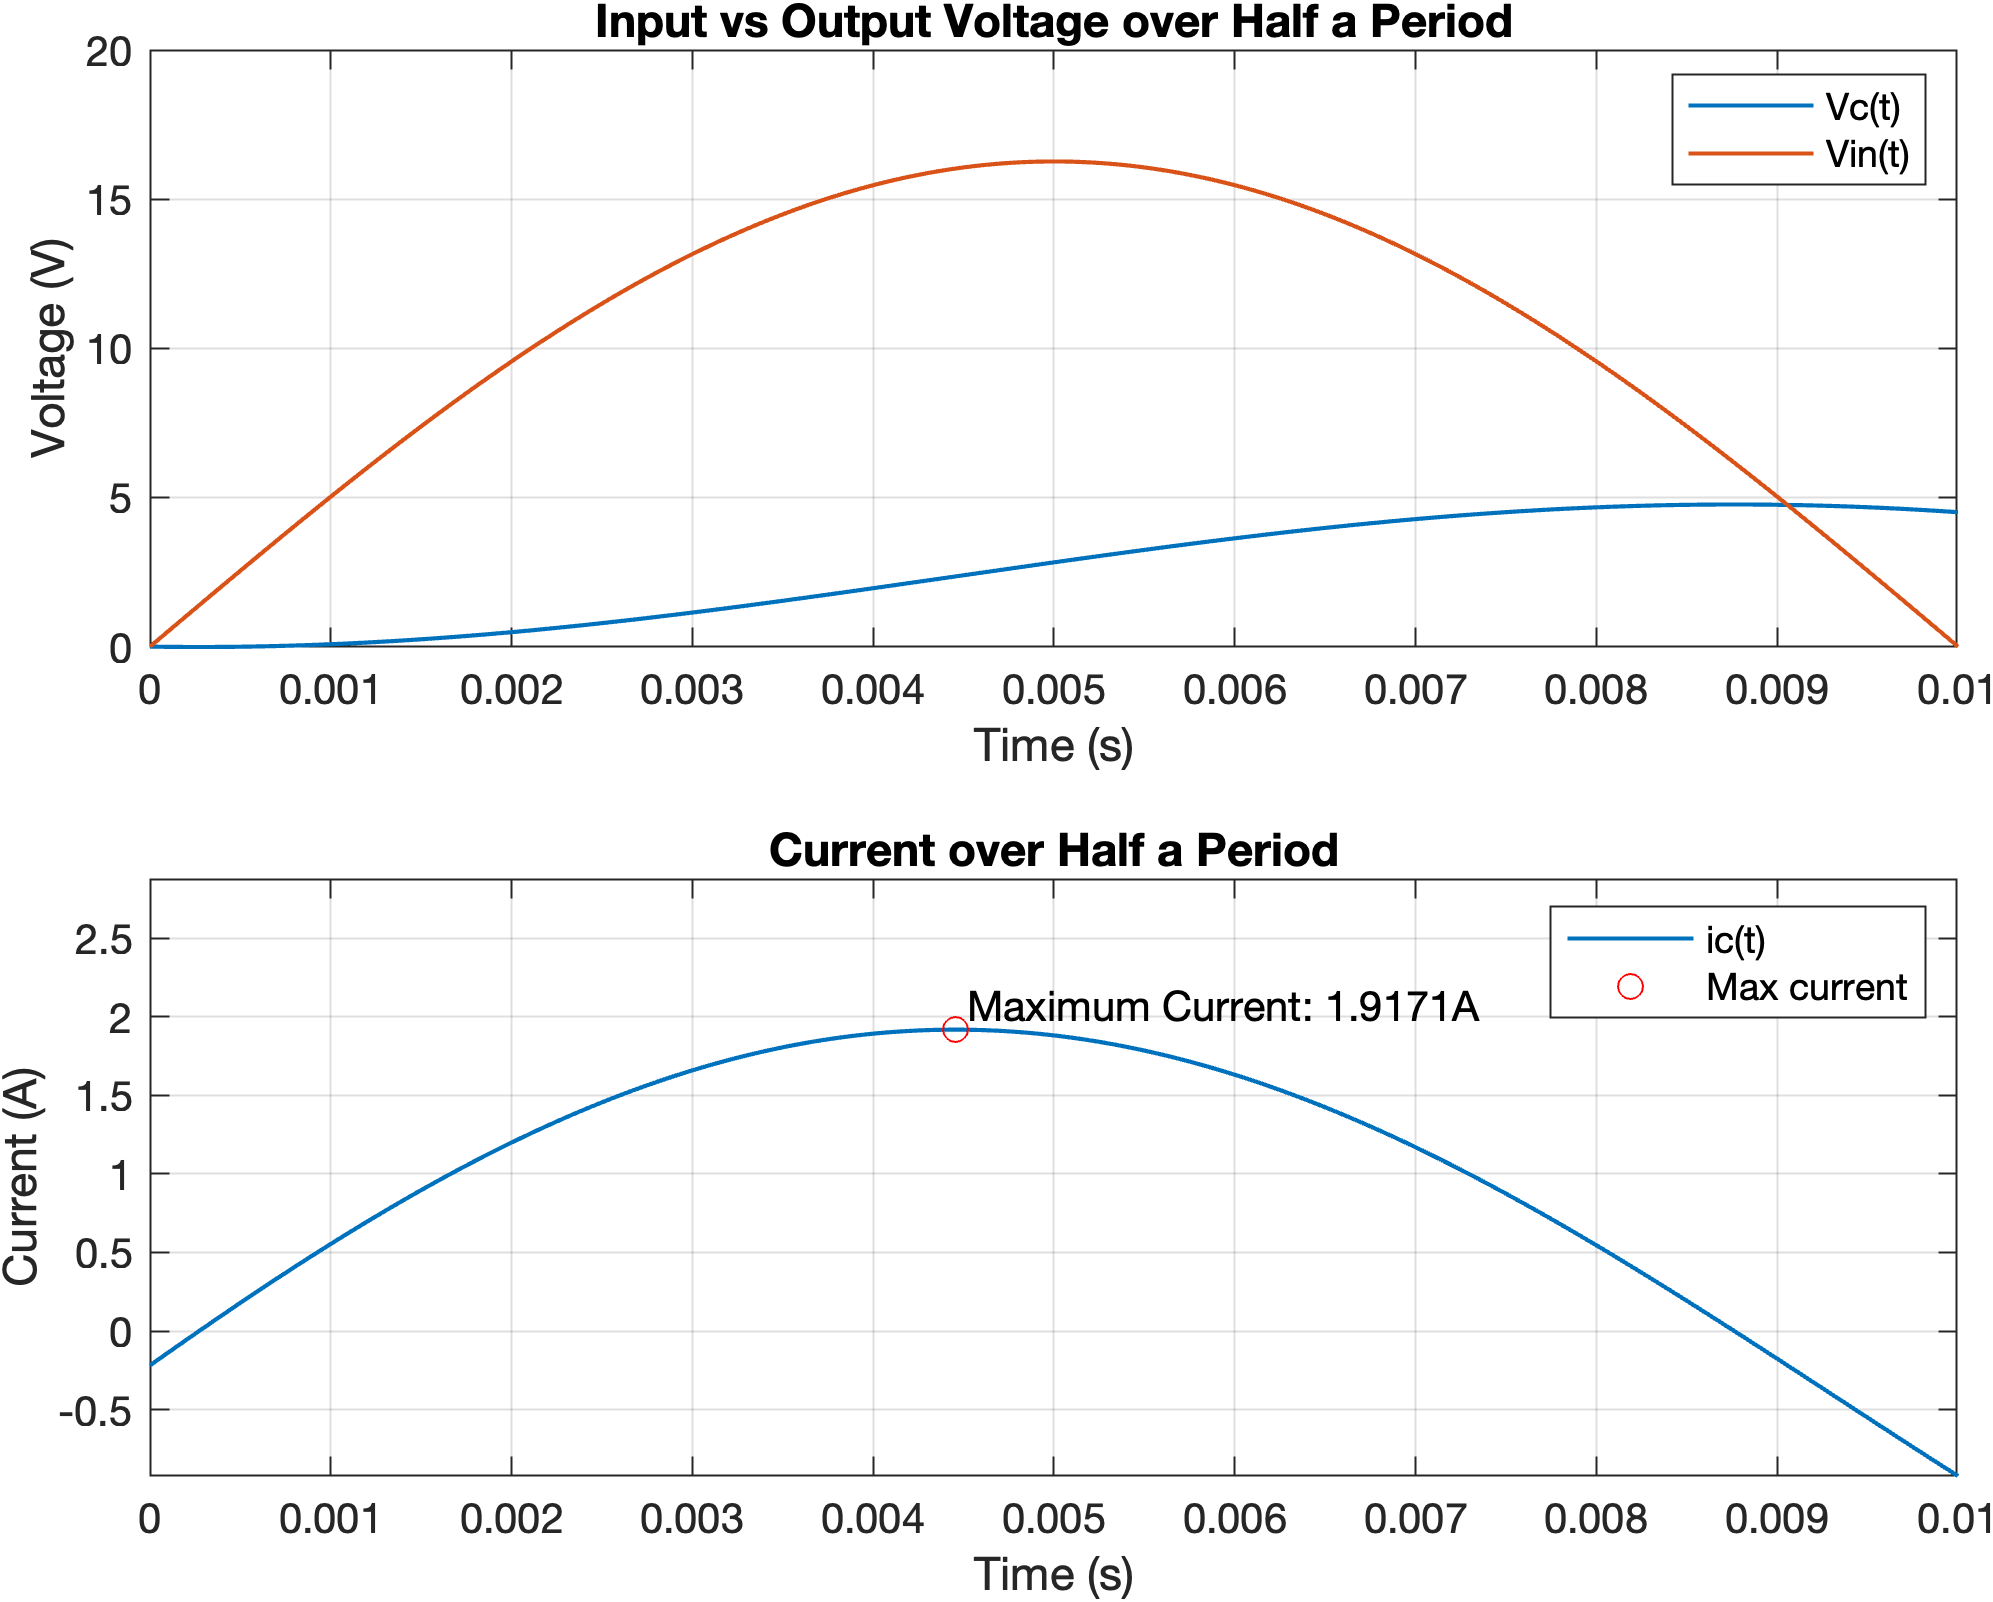
\includegraphics[width=\textwidth]{graphics/diode_current.png}
	\caption{$V_c(t)$ and $i_c(t)$ plot over a half period}
	\label{fig:diode_current}
\end{figure}
The graph above gives a reasonable approximation of the maximum current $1.917A$ flowing through the signal diode in forward bias. The piece-wise linear diode model approximates the behaviour of the Shockley diode for a current range up to $\simeq 3.834A$.

\pagebreak
\subsubsection{Zener Diode} An ideal zener diode behaves like an ideal diode for $v > -V_z$. At $v = -V_z$ it conducts current in the reverse direction. A zener diode can be modelled in the reverse breakdown region by the series combination of a voltage source $V_z$ and resistance $r_z$. 
\\

The piece-wise linear approximation of the ideal diode can be applied to the zener resulting in
\begin{figure}[H]
    \centering
    \begin{circuitikz}[american voltages] \draw
 	(0,5) node[label=A] {} to[ZZener diode,o-o,l=$V_z$,i=$i_z$] (0,0)
	(3,5) node[label=A] {} to[battery1,o-,l=$V_{z}$] (3,4) 
	(3,4) to[R, l=$R_z$, i_=$i_z$] (3,1)
	(3,1) to[nos,o-o] (3,0);
\end{circuitikz}
    \caption{Piece-wise linear diode approximation of the zener diode}
    \label{fig:piecewise_zener}
\end{figure}

The resulting i-v characteristic is the same as the ideal diode,
\begin{equation}
    i_z = \begin{cases}
        \bracket{\frac{V_{A} - V_{z}}{R_z}} \hspace{1cm} &V_{A} \geq V_z \\
        0 \hspace{1cm}   &V_{A} < V_z
    \end{cases}
\end{equation}
